\documentclass{beamer}

\usepackage{pslatex}
\usepackage{graphicx}
\usepackage[utf8]{inputenc}
\usepackage{amssymb}            % Principaux symboles
%\usepackage{fontspec}
%\usepackage{xunicode}
%\usepackage{xltxtra}
\usepackage[frenchb]{babel}
%\defaultfontfeatures{Scale=MatchLowercase}
%\setmainfont[Mapping=tex-text,Ligatures={Common, Historical}]{Linux Libertine O}
%\setsansfont[Mapping=tex-text]{Linux Biolinum O}
%\setmonofont[Scale=0.75]{DejaVu Sans Mono}

%% Packages pour le texte
\usepackage[misc,geometry]{ifsym}	% Police numéros battons
\usepackage{pifont}		% Police \ding
\usepackage{eurosym}		% Symbole de l'euro
\usepackage{soul}		% Souligner
\usepackage{enumerate}		% Listes
\usepackage{verbatim}		% Codes source
\usepackage{moreverb}		%	et listings
\usepackage{textcomp}
\usepackage{multicol}

%% Packages pour les tableaux
\usepackage{array}		% Outils supplémentaires
\usepackage{multirow}		% Colonnes multiples
\usepackage{tabularx}		% Largeur totale donnée
\usepackage{longtable}		% Sur plusieurs pages

%% Les packages pour les dessins
\usepackage{graphicx}		% Insertion de figures
%\usepackage{picins}		% Dans un paragraphe
\usepackage{epic}		% Capacités graphiques
\usepackage{eepic}		% 	étendues
\usepackage{afterpage}		% Voir page 69
\usepackage{rotating}		% Tourner du texte
\usepackage{caption}		% Légendes
% \addto\captionsfrench{\def\figurename{}}

%% Packages pour les maths
\usepackage{amsmath}		% Commandes essentielles
\usepackage{amssymb}		% Principaux symboles
\usepackage{mathrsfs}		% Police calligraphique
\usepackage{theorem}		% Théorèmes
%\usepackage{tikz}		% Courbes
\usepackage{esvect}             % Vecteurs
%\usetikzlibrary{shapes,arrows,shadows}
\usepackage{pgf}
%\usetikzlibrary{arrows}
% Packages pour la physique
\usepackage{sistyle}		% Unités
\usepackage[version=3]{mhchem}	% Formules chimiques
\usepackage{etex}
\usepackage{m-pictex,m-ch-en}

%\usepackage{media9}
\usepackage{multimedia}		% Vidéos dans la présentation
%\usepackage{movie15}

\usepackage{ccicons}		% Licence creativecommons

\SIdecimalsign{,}


\AtBeginSection[]
{
  \begin{frame}
    \frametitle{sommaire}
    \begin{multicols}{2}
      {\small
        \tableofcontents[currentsection, hideothersubsections]}
    \end{multicols}
  \end{frame}
}

\usetheme{Warsaw}



\usepackage{tikz}
\usepackage{pgfplots}
\usepackage{adjustbox}
\usepackage{colortbl}
\usepackage{subfigure}
\usepackage{parcolumns}

\useoutertheme{infolines}
\setbeamersize{text margin left=1cm,text margin right=1cm}
\usetikzlibrary{arrows}
\definecolor{qqwuqq}{rgb}{0,0.39,0}
\definecolor{xdxdff}{rgb}{0.49,0.49,1}
\definecolor{uququq}{rgb}{0.25,0.25,0.25}
\definecolor{qqqqff}{rgb}{0,0,1}
\definecolor{red}{rgb}{1,0,0}
\definecolor{yel}{rgb}{1,1,0}
\definecolor{sky}{rgb}{0.2,0.2,1}
\setcounter{tocdepth}{4}
\newcolumntype{M}{>{$\vcenter\bgroup\hbox\bgroup}c<{\egroup\egroup$}}
\setlength{\arrayrulewidth}{2pt}
\setlength{\extrarowheight}{0pt}
\setlength{\tabcolsep}{0pt}

\title{Comment simuler numériquement la géomorphologie alpine ?}
\subtitle{Présentation du TPE}
\author{Gros Alexis, Manceau Thibaut, Porteries Tristan}
%\logo{
\includegraphics[height=0.5cm]{blender.png}}

\begin{document}
\CenterWallPaper{1}{Images/inde.jpg}
% Titre
\frame{\titlepage}

\begin{frame}
    \frametitle{Sommaire}
    \begin{multicols}{2}
      {
				\setcounter{tocdepth}{1}
        \tableofcontents
      }
    \end{multicols}
\end{frame}

\section{Les principes géomorphologiques}

\subsection{Glossaire}
\begin{frame}{Glossaire géomorphologique}
  \begin{description}
    \item[Géomorphologie :] Étude de la genèse des reliefs.
    \item[Plaque litosphérique :] Partie supérieure des plaques tectoniques terrestres ou maritimes.
    \item[Asténosphere :] Partie inférieure des plaques tectoniques, siège des séismes de profondeurs.
    \item[Obduction :] Une plaque en chevauche une autre.
  \end{description}
  \begin{center}
    \begin{figure}
      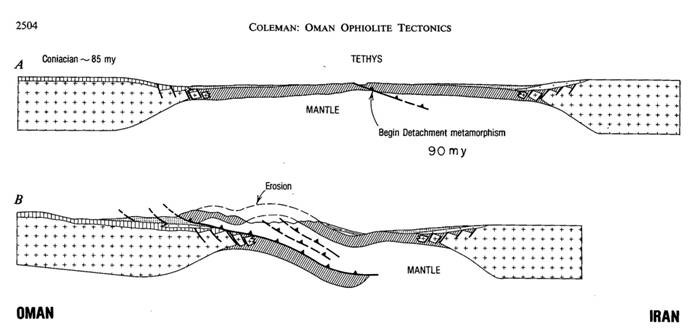
\includegraphics[width=6cm]{Images/Images_Alexis/image007.jpg}
      \caption{Exemple d'obduction}
    \end{figure}
  \end{center}
\end{frame}

\subsection{Les plaques tectoniques}
\begin{frame}{Introduction à la tectonique des plaques}
  \begin{center}
    \begin{figure}
      \subfigure[Carte des principales plaques tectoniques]{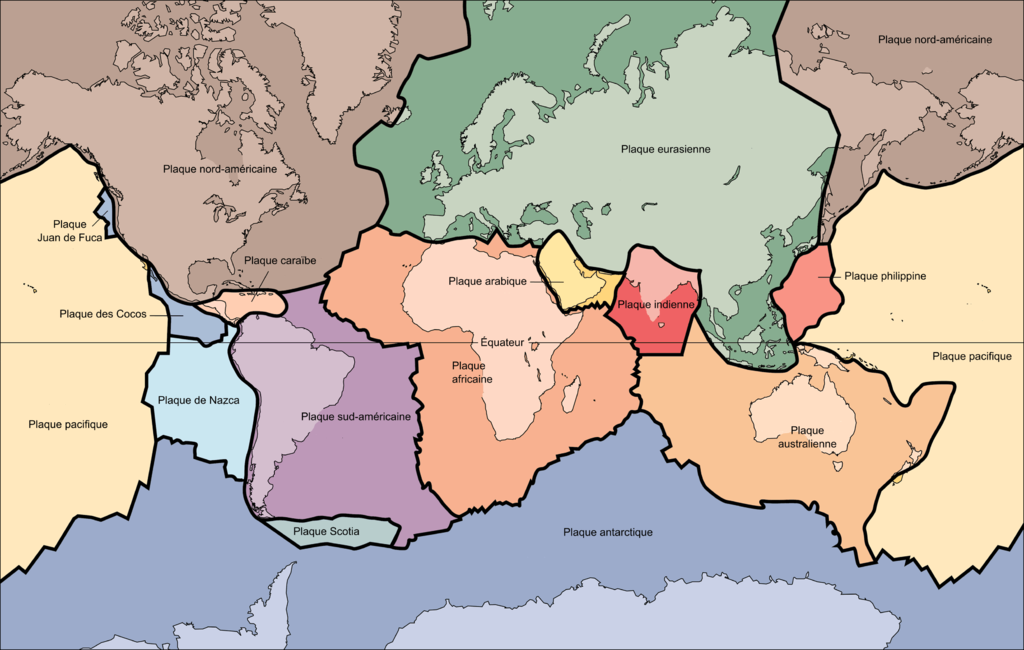
\includegraphics[width=4cm]{Images/Images_Alexis/plaques.png}}
    \end{figure}
    \begin{figure}
      \subfigure[Les Andes]{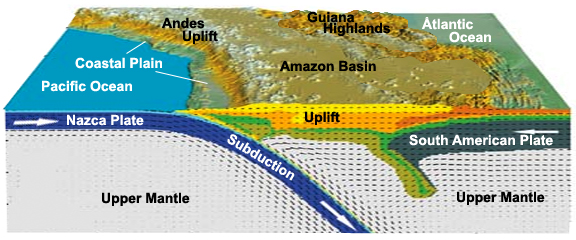
\includegraphics[width=4cm]{Images/Images_Alexis/andes.jpg}}
      \subfigure[Le Japon]{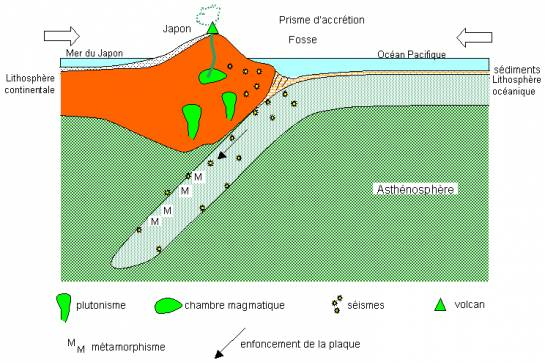
\includegraphics[height=3cm]{Images/Images_Alexis/japon.jpg}}
    \end{figure}
  \end{center}
\end{frame}

\section{Les altérations}
\subsection{Les altérations physiques}
\begin{frame}
  \begin{center}
    \begin{figure}
      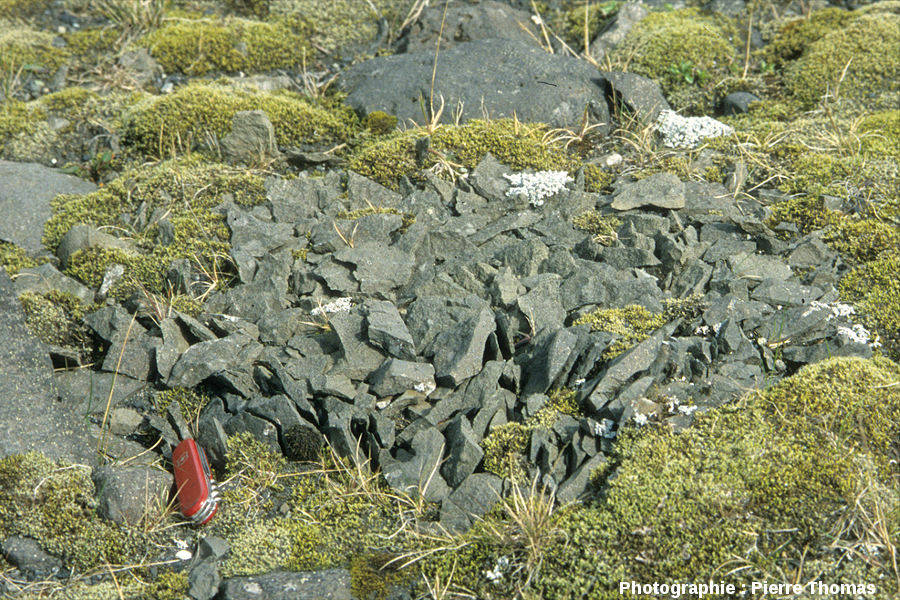
\includegraphics[width=6cm]{Images/Diapos/Alteration/Physique/cryoclastie.jpg}
      \caption{Exemple du phénomène de cryoclastie}
    \end{figure}
  \end{center}
\end{frame}

\subsection{Les altérations chimiques}
\begin{frame}
  \begin{center}
    \begin{figure}
      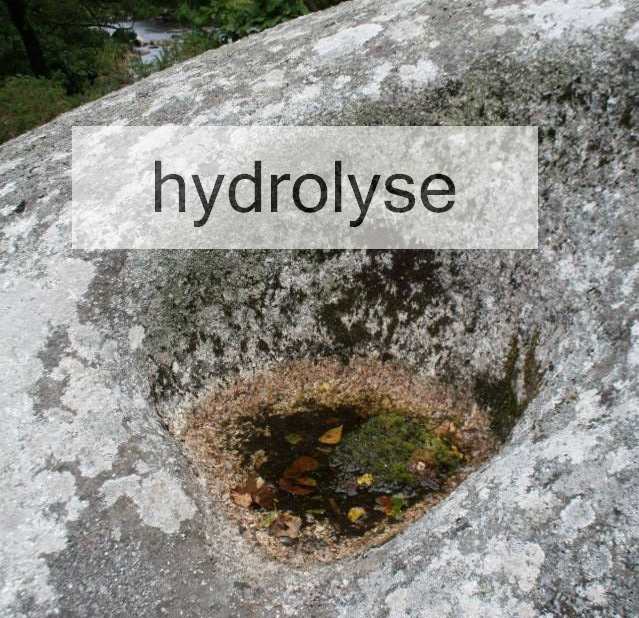
\includegraphics[width=5cm]{Images/Diapos/Alteration/Chimiques/hydrolyse.jpeg}
    \end{figure}
  \end{center}
\end{frame}

\section{L'érosion}

\subsection{Ruissellement et érosion fluviale}
\begin{frame}
 \begin{center}
  \begin{figure}
    \subfigure[Les « Badlands »]{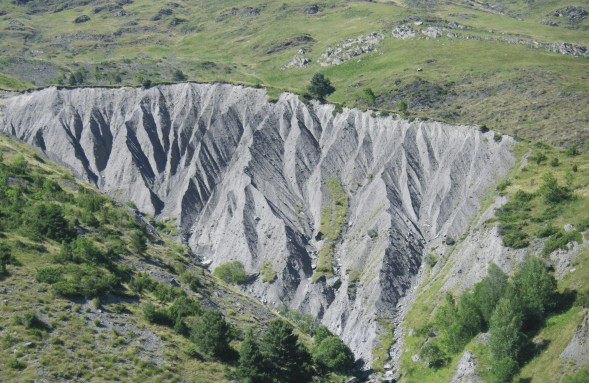
\includegraphics[height=3cm]{Images/Diapos/Erosion/Fluviale/bad_lands.jpg}}
    \subfigure[Schéma de l'érosion verticale]{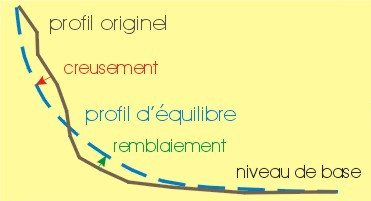
\includegraphics[height=3cm]{Images/Diapos/Erosion/Fluviale/n_base.jpg}}
  \end{figure}
 \end{center}
\end{frame}

\subsection{L'érosion karstique}
\begin{frame}
  \begin{center}
    \begin{figure}[h]
      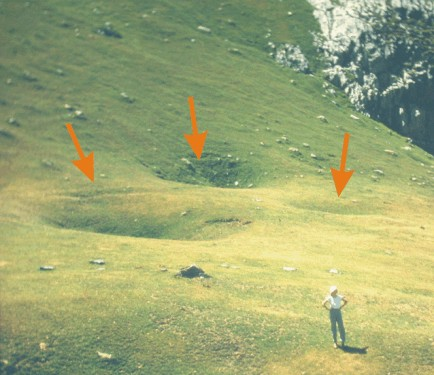
\includegraphics[width=5.35cm]{Images/Diapos/Erosion/Karstique/dolines.jpg}
      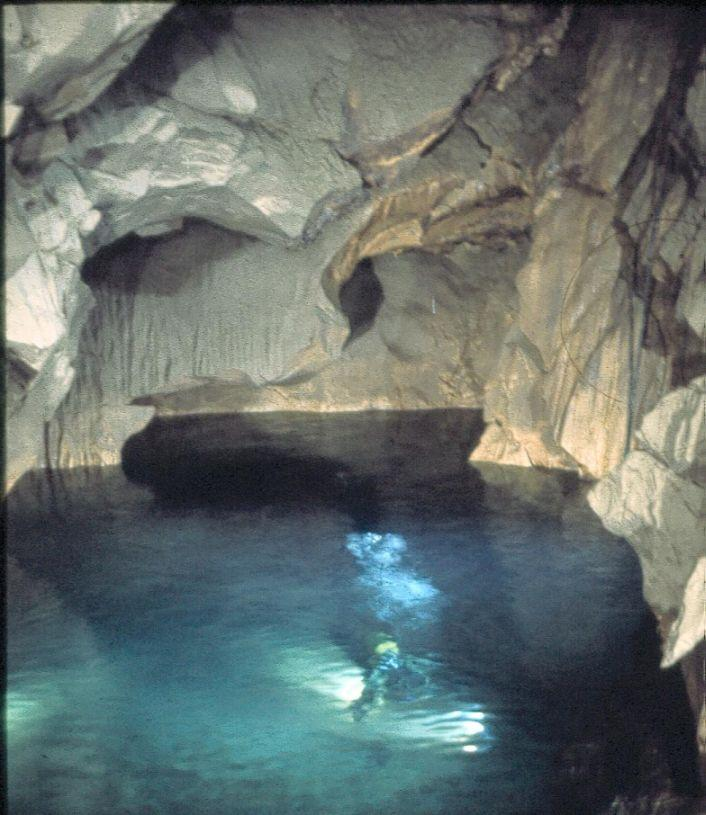
\includegraphics[width=4cm]{Images/Diapos/Erosion/Karstique/erosion-karstique-fig04.jpg}
      \caption{Dolines et grottes souterraines}
    \end{figure}
  \end{center}
\end{frame}

\subsection{L'érosion glaciaire}
\begin{frame}
  \begin{center}
    \begin{figure}
      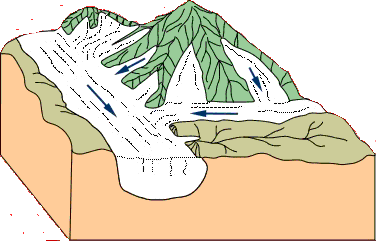
\includegraphics[width=7cm]{Images/Diapos/Erosion/Glaciaire/Erosion_glaciaire_Bourque4B.png}
      \caption{Schéma de l'érosion glaciaire}
    \end{figure}
  \end{center}
\end{frame}

\section{Problématiques géologiques des Alpes}

\subsection{L'historique des Alpes}
\begin{frame}{Chronologie des Alpes}
  \begin{itemize}
    \item \textit{-200 Ma, trias} : ouverture de l’océan alpin ;
    \item \textit{-140 Ma, crétacé inférieur} : début de la compression de l’océan alpin ;
    \item \textit{-65 Ma, paléocène} : émersion de la plate-forme continentale, le mont blanc passe sous la zone d'obduction pour ressurgir ensuite ;
    \item \textit{-23 Ma, néogène}: création du jura ;
    \item \textit{Pliocène} : séparation de la couche calcaire du reste des plis.
  \end{itemize}
  \begin{center}
    \begin{figure}
      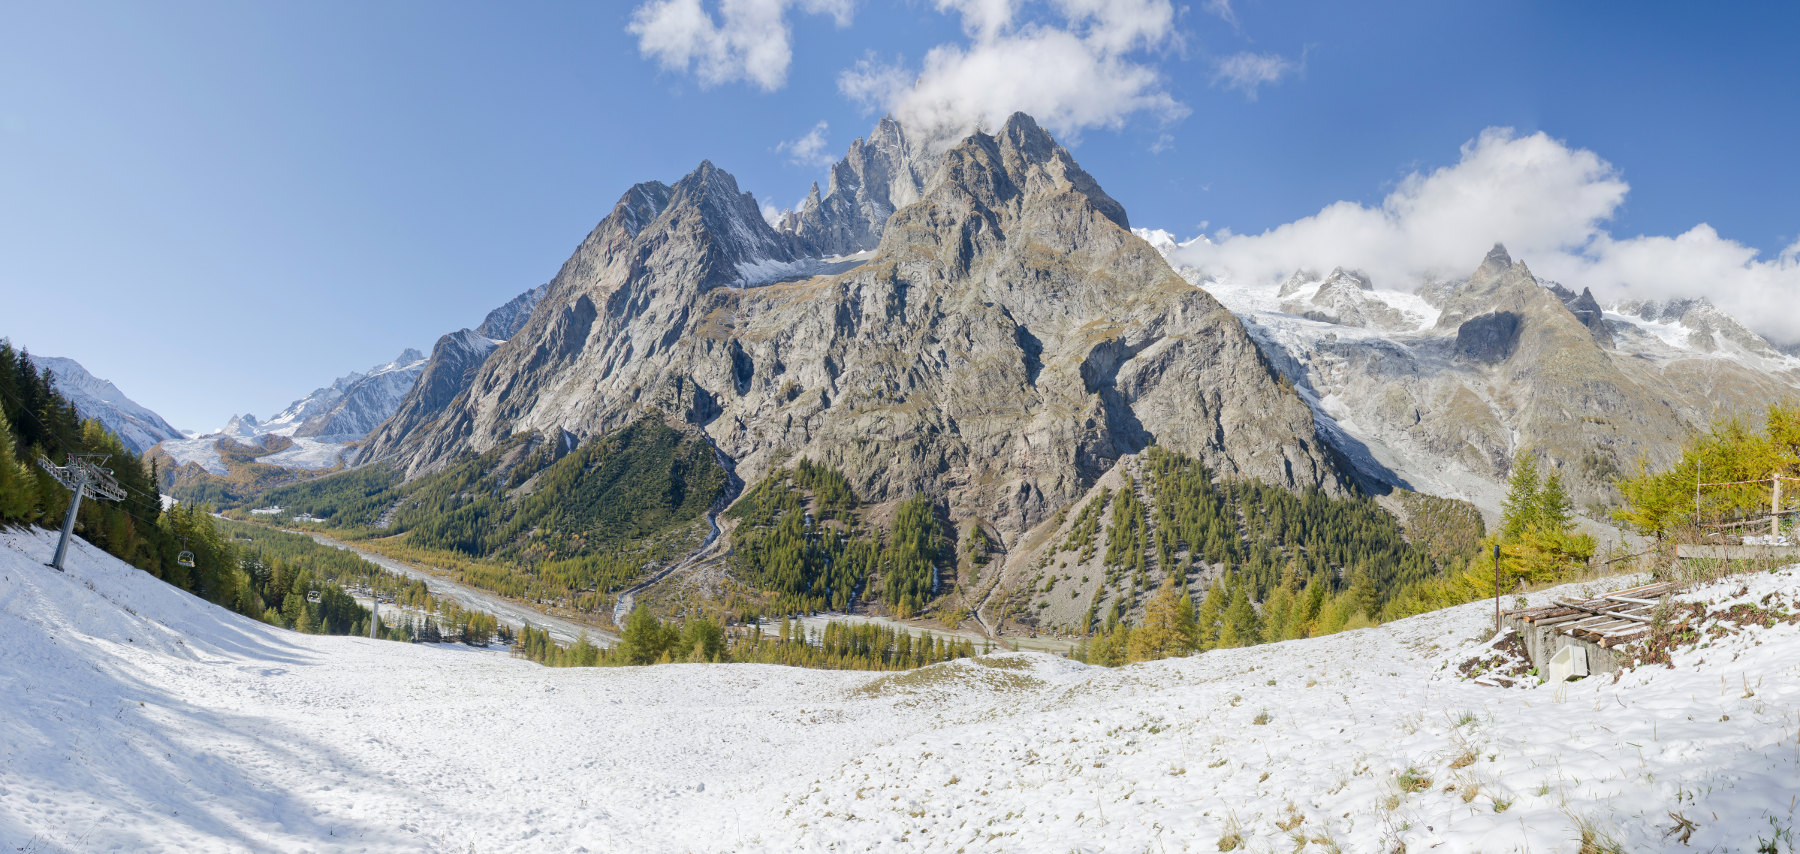
\includegraphics[width=4cm]{Images/Images_Alexis/mont_blanc.jpg}
    \end{figure}
  \end{center}
\end{frame}

\subsection{Les glaciers}
\begin{frame}{L'effet des glaciers sur le paysage Alpin}
  \begin{center}
    \begin{figure}
      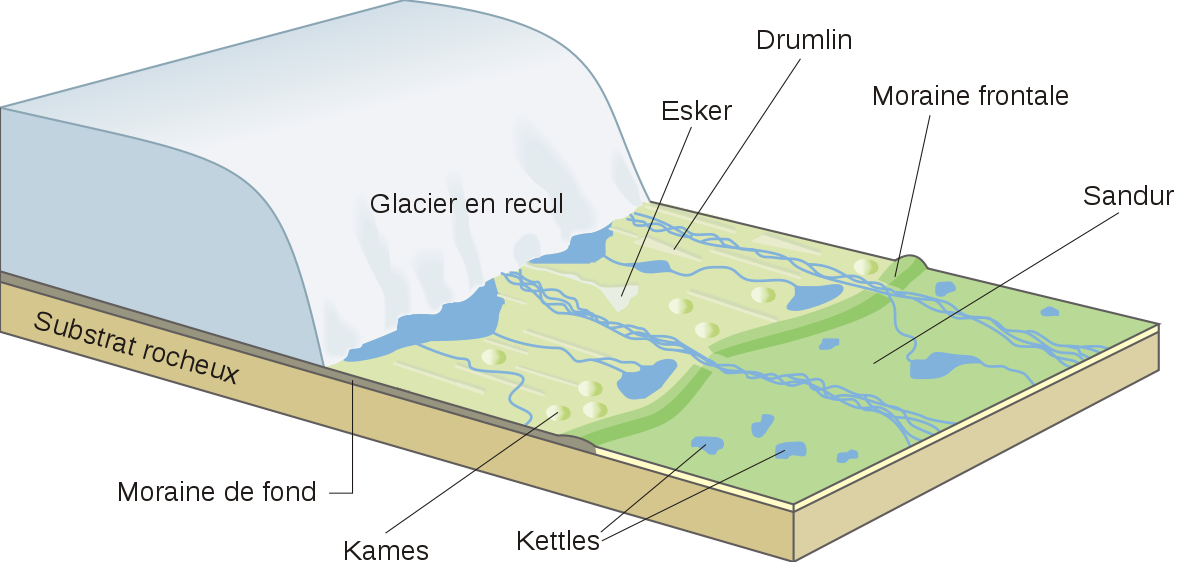
\includegraphics[height=2cm]{Images/Images_Alexis/glacier_reculon.png}
      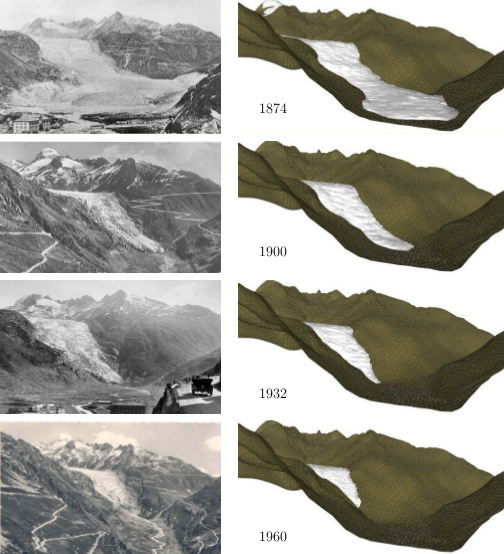
\includegraphics[height=2cm]{Images/Images_Alexis/glaciers_img3.png}
      \caption{Les ères glaciaires successives ont grandement participé au façonnage de nos paysages.}
      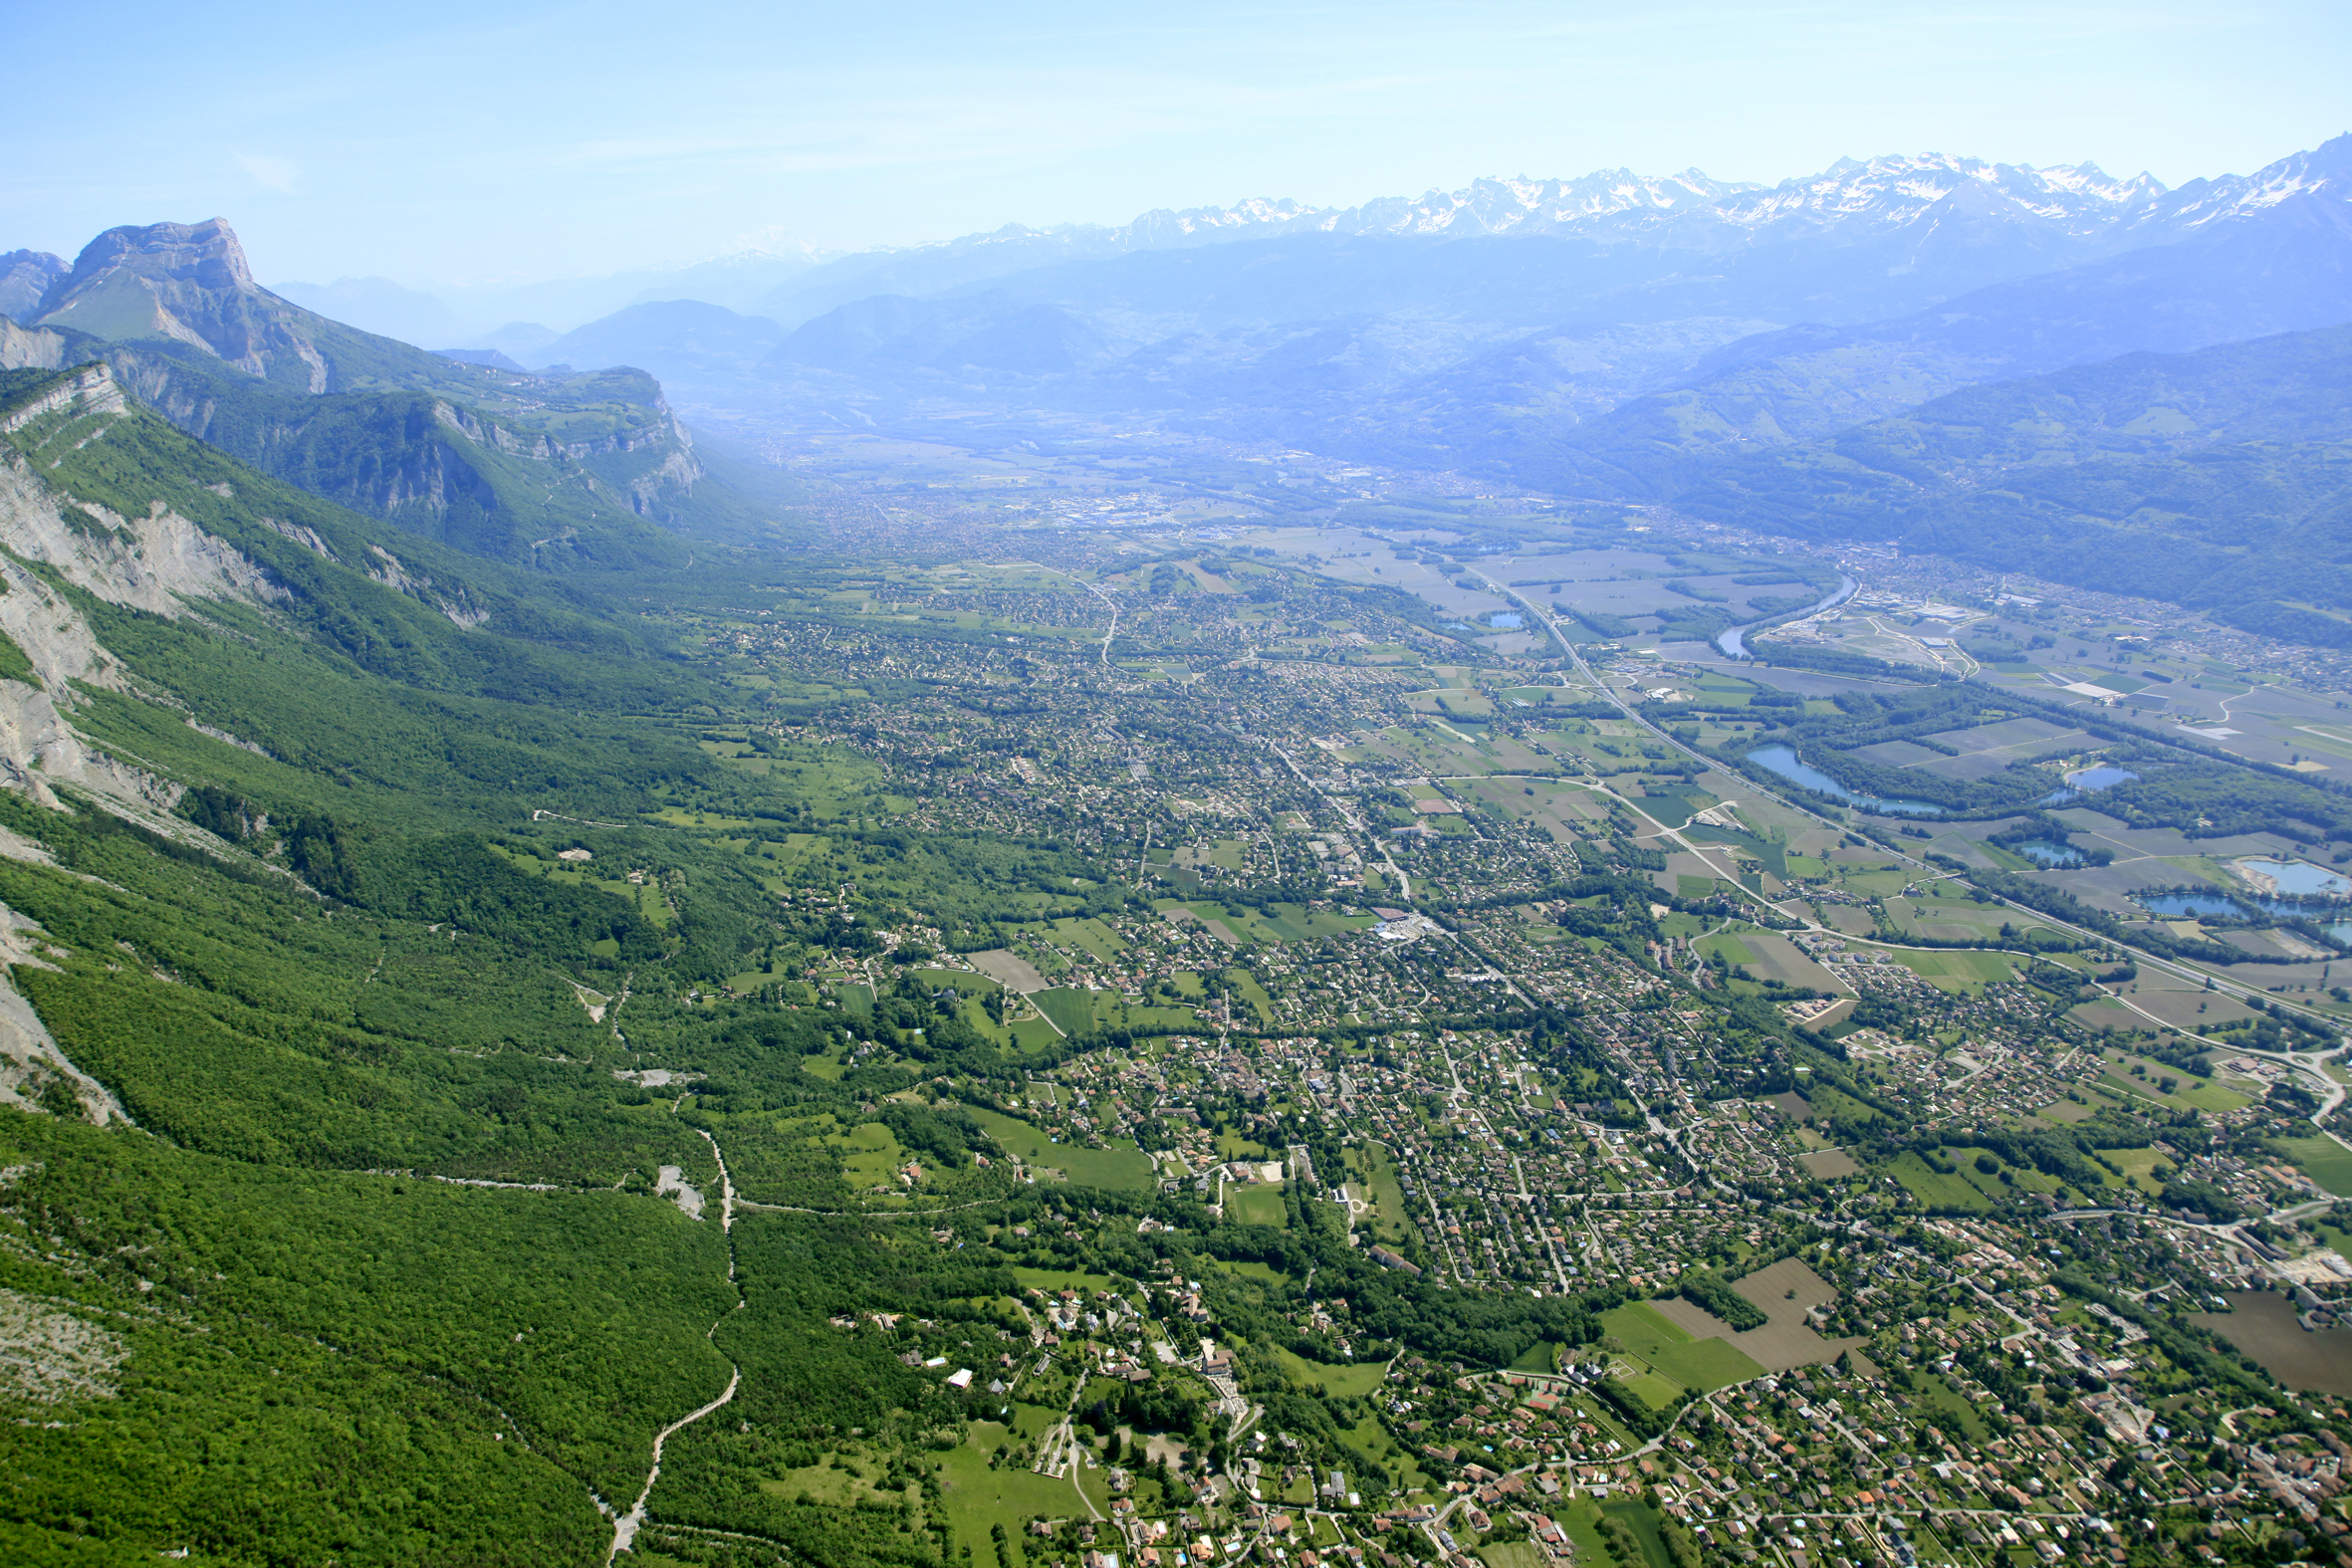
\includegraphics[width=4cm]{Images/Images_Alexis/gresivaudan.jpg}
    \end{figure}
  \end{center}
\end{frame}


\section{Les simulations alternatives}
\subsection{Le bruit de perlin}
\begin{frame}{Bruit de perlin}
  \begin{center}
    \begin{figure}
      \subfigure[Représentation du bruit de perlin]{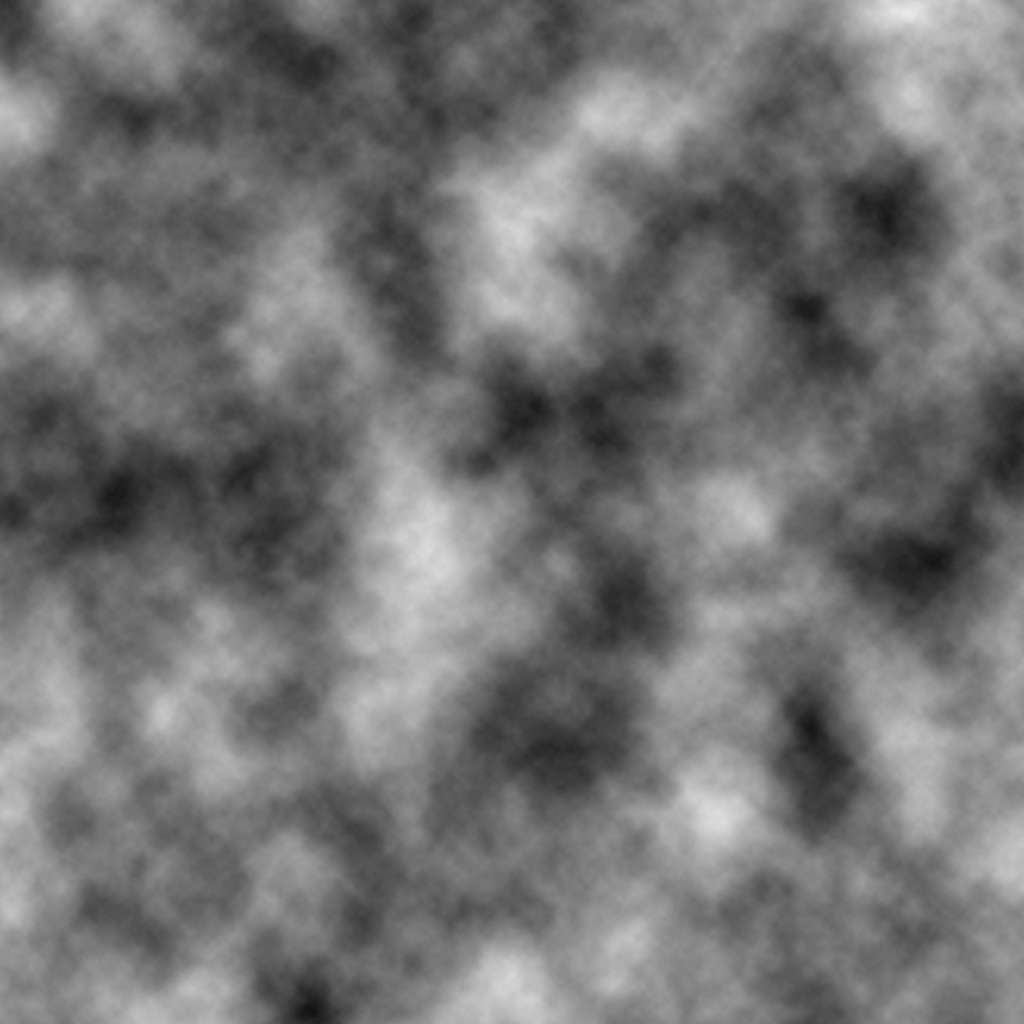
\includegraphics[height=4cm]{Images/Images_Alexis/perlin_noise.png}}
      \subfigure[Paysage généré grâce à un bruit de perlin fractalisé]{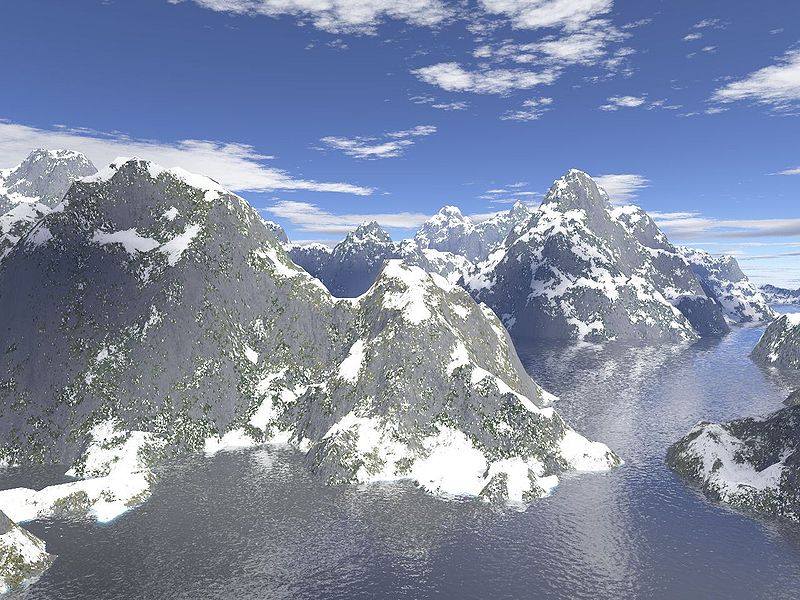
\includegraphics[height=4cm]{Images/Images_Alexis/fractal&shader.jpg}}
      \caption{Différentes représentation du bruit de perlin}
    \end{figure}
  \end{center}
\end{frame}

\subsection{Les cellules de voronoi}
\begin{frame}{Cellules de Voronoi}
  \begin{center}
    \begin{figure}
      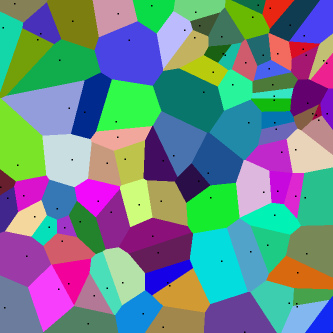
\includegraphics[width=5cm]{Images/Images_Alexis/voronoi.png}
      \caption{Représentation des cellules de voronoi.}
    \end{figure}
  \end{center}
\end{frame}

\subsection{Les voxels et boxel}
\begin{frame}{Présentation de voxels et boxel}
  \begin{center}
    \begin{figure}
      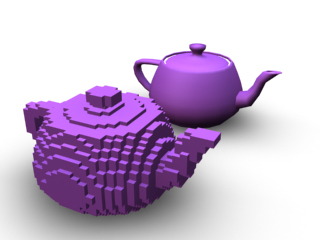
\includegraphics[width=5cm]{Images/Images_Alexis/voxel_teapot.jpg}
      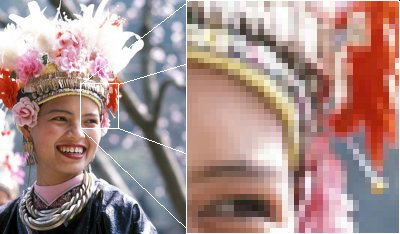
\includegraphics[width=5cm]{Images/Images_Alexis/example_matricielle.jpg}
    \end{figure}
    \begin{figure}
      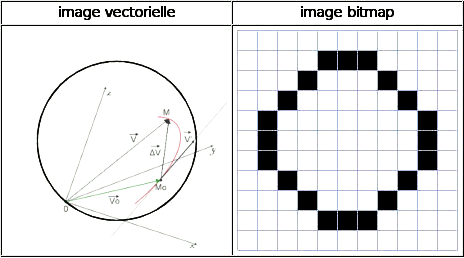
\includegraphics[width=5cm]{Images/Images_Alexis/comparaison_vecteur_matrice.png}
    \end{figure}
  \end{center}
\end{frame}

\begin{frame}{Démonstration des voxels}
  \begin{center}
    \begin{figure}
      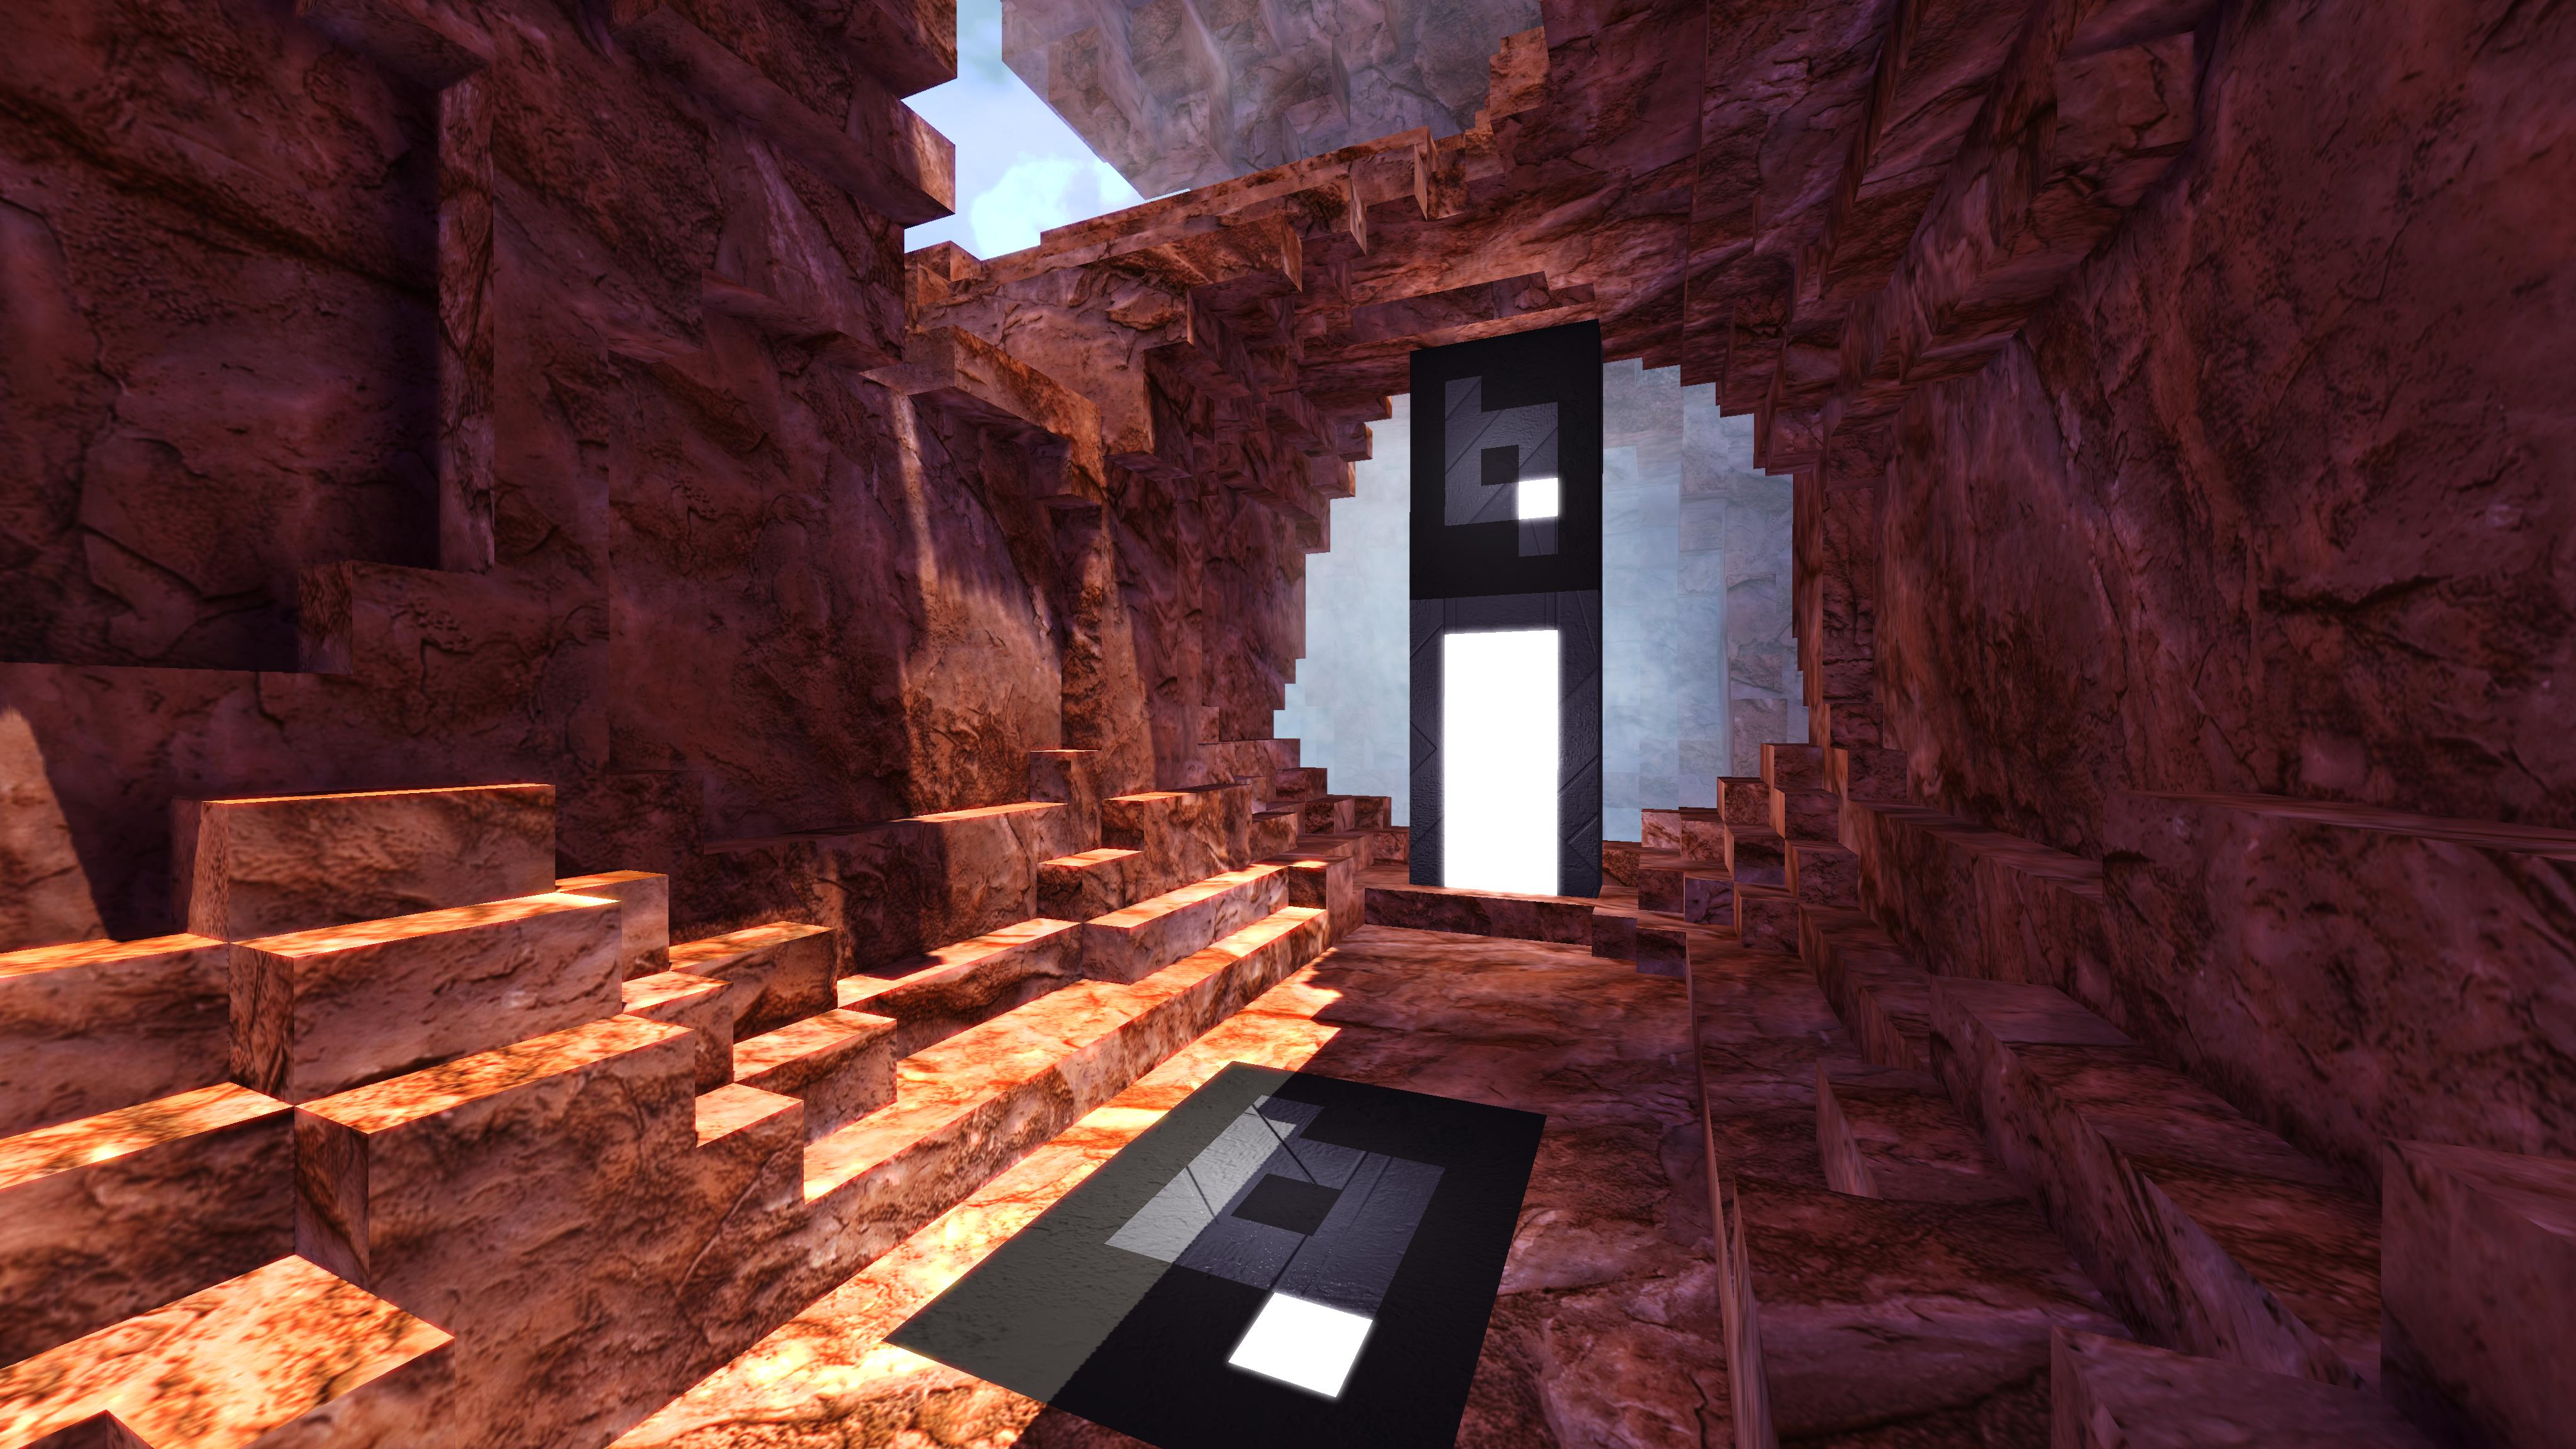
\includegraphics[height=3cm]{Images/Images_Alexis/voxel_engine3.jpg}
      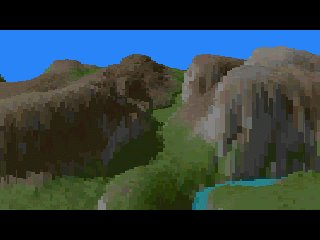
\includegraphics[height=3cm]{Images/Images_Alexis/voxel_engine1.jpg} \\
      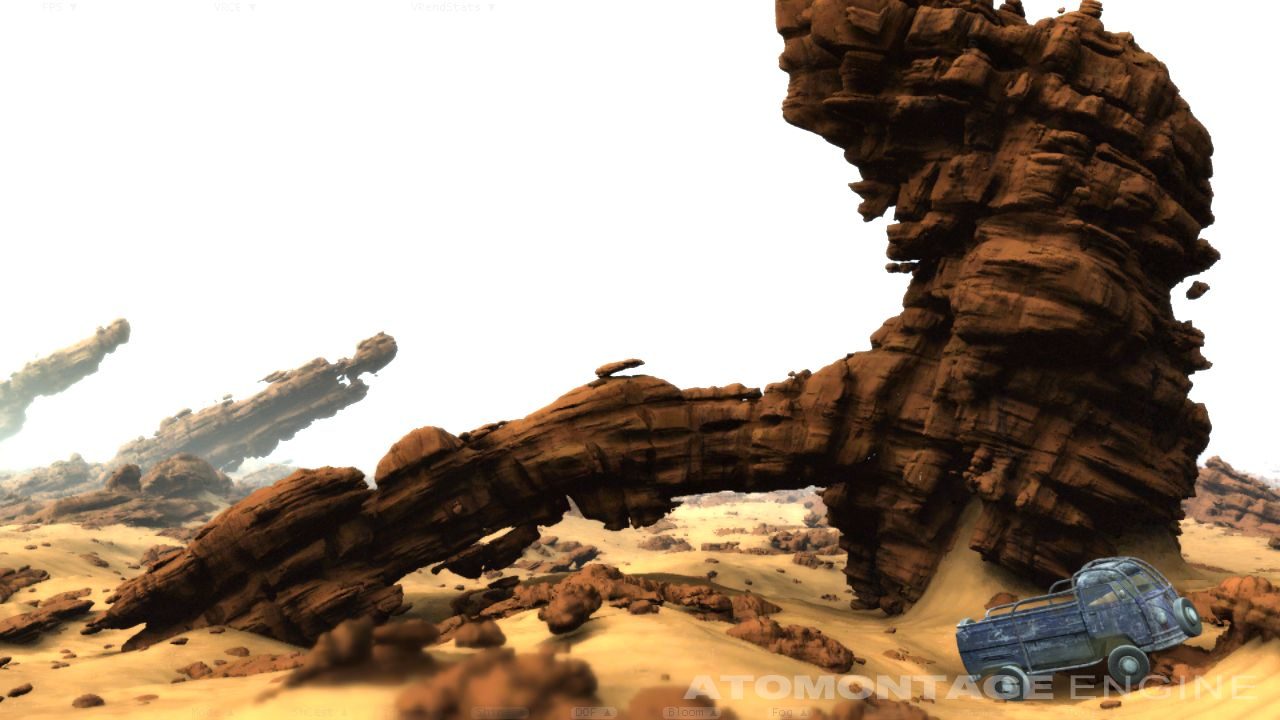
\includegraphics[height=3cm]{Images/Images_Alexis/voxel_engine4.jpg}
      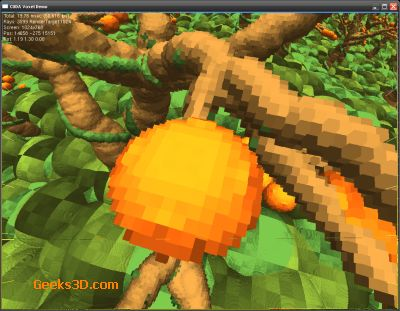
\includegraphics[height=3cm]{Images/Images_Alexis/voxel_engine2.jpg}
      \caption{Exemples d'applications des voxels}
    \end{figure}
  \end{center}
\end{frame}

\subsection{Les simulations physiques}
\begin{frame}{Simulation physique par pâtes}
  \begin{center}
    \begin{figure}
      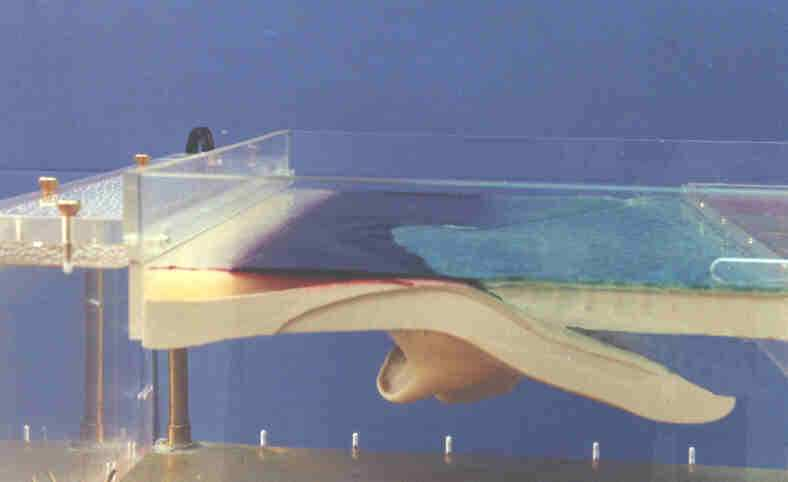
\includegraphics[width=7cm]{Images/simulation_physique.png}
      \caption{Photo de simulation physique par pâtes}
    \end{figure}
  \end{center}
\end{frame}

\subsection{Les simulations numériques}
\begin{frame}{Simulation numérique}
  \begin{center}
    \begin{figure}
      \subfigure[Simulation après 3100 pas de simulation]{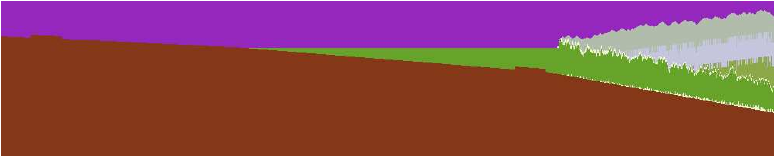
\includegraphics[width=10cm]{Images/3100_cell.png}}
      \subfigure[Simulation après 7100 pas de simulation]{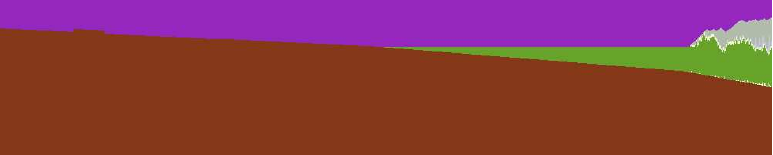
\includegraphics[width=10cm]{Images/7100_cell.png}}
      \caption{Source: Publication scientifique}
    \end{figure}
  \end{center}
\end{frame}

\section{La simulation cellulaire}

\subsection{Les cellules}
\begin{frame}{Définition d'une cellule}
  \begin{tabular}{m{8cm}m{1cm}m{2cm}}
    \mbox{Cellule : plus petit élément incompressible. Taille}
    \mbox{réelle : sphère de 10 m de Ø Taille dans la}
    \mbox{simulation : sphère de Ø 1} &&
    
\includegraphics[width=1.5cm]{Images/cellule.png}
  \end{tabular}
  Propriétés mutables :
  \begin{itemize}
   \item vélocité~;
   \item position~;
   \item cellules adjacentes.
  \end{itemize}
  Propriétés immuables :
  \begin{itemize}
   \item plaque tectonique.\\
  \end{itemize}
  \smallbreak
  Cellules en collision : deux cellules en interaction n'ayant pas la même plaque.
\end{frame}

\begin{frame}{Représentation graphique des cellules}
  \begin{figure}
    \subfigure[Cellule inactive.]{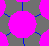
\includegraphics[height=2.8cm]{Images/cellule_violet.png}}
    \subfigure[Cellule du front.]{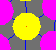
\includegraphics[height=2.8cm]{Images/cellule_jaune.png}}
    \subfigure[Cellule en collision.]{
\includegraphics[height=2.8cm]{Images/cellule_noir.png}}
    \caption{Représentation graphique de tous les états d'une cellule. Les interactions sont symbolisées par des lignes bleues.}
  \end{figure}
\end{frame}

\begin{frame}{Disposition des cellules}
  Disposition en nid-d'abeille sur un plan au lancement de la simulation. Equidistance « parfaite » de 1 entre les cellules.
  \begin{center}
    \begin{figure}
      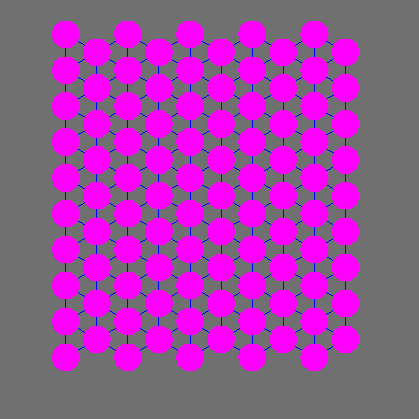
\includegraphics[width=5cm]{Images/hexagone.png}
      \caption{Image de la simulation juste après la création et la disposition des cellules}
    \end{figure}
  \end{center}
\end{frame}

\subsection{Les interactions}
\begin{frame}{Différentes interactions entre cellules}
\begin{figure}
\begin{center}
\begin{tikzpicture}[line cap=round,line join=round,>=triangle 45,x=1.0cm,y=1.0cm,scale=0.5,every node/.style={scale=0.8}]
\clip(-2.25,-2.25) rectangle (21.25,6);
\draw[red](0,2.83) circle (2cm);
\draw(2.83,0) circle (2cm);
\draw[red](7,2.83) circle (2cm);
\draw(9.83,0) circle (2cm);
\draw[red](15,2) circle (2cm);
\draw(19,2) circle (2cm);
\draw[yel] [->] (0,2.83) -- (0,1);
\draw [->] (2.83,0) -- (4.09,-1.26);
\draw [->] (9.83,0) -- (8.75,1.09);
\draw[yel] [->] (7,2.83) -- (7,4.83);
\draw[yel] [->] (15,2) -- (15,4);
\draw [->] (19,2) -- (19,3);
\begin{scriptsize}
\fill [color=red] (0,2.83) circle (1.5pt);
\draw[color=red] (0.42,3.21) node {$C_1$};
\fill [color=qqqqff] (2.83,0) circle (1.5pt);
\draw[color=qqqqff] (3.27,0.36) node {$C_2$};
\fill [color=red] (7,2.83) circle (1.5pt);
\draw[color=red] (7.42,3.21) node {$C_1$};
\fill [color=qqqqff] (9.83,0) circle (1.5pt);
\draw[color=qqqqff] (10.24,0.36) node {$C_2$};
\fill [color=red] (15,2) circle (1.5pt);
\draw[color=red] (15.42,2.36) node {$C_1$};
\fill [color=qqqqff] (19,2) circle (1.5pt);
\draw[color=qqqqff] (19.44,2.36) node {$C_2$};
\draw[color=black] (0.19,2.13) node {$u$};
\draw[color=black] (3.61,-0.35) node {$?$};
\draw[color=black] (9.66,0.6) node {$?$};
\draw[color=black] (7.14,4.04) node {$u$};
\draw[color=black] (14.91,3.21) node {$u$};
\draw[color=black] (18.63,2.73) node {$?$};
\end{scriptsize}
\end{tikzpicture}
\end{center}
\caption{Trois interactions différentes entre cellules : 1) Compression ; 2) Traction ; 3) Friction.}
\end{figure}
\end{frame}

\begin{frame}{Centre instantané de rotation}
  \begin{minipage}{\dimexpr.55\textwidth-\tabcolsep-.5pt}
    \begin{center}
      \begin{tikzpicture}[line cap=round,line join=round,>=triangle 45,x=0.4cm,y=0.4cm,scale=0.7,every node/.style={scale=0.7}]
      \clip(-5,-5) rectangle (17,12);
      \draw [shift={(16.25,7)},color=qqwuqq,fill=qqwuqq,fill opacity=0.1] (0,0) -- (-150.26:4.15) arc (-150.26:-139.13:4.15) -- cycle;
      \draw [shift={(16.25,7)},color=qqwuqq,fill=qqwuqq,fill opacity=0.1] (0,0) -- (180:4.15) arc (180:191.31:4.15) -- cycle;
      \draw[color=qqwuqq,fill=qqwuqq,fill opacity=0.1] (0.88,7) -- (0.88,7.88) -- (0,7.88) -- (0,7) -- cycle; 
      \draw[color=qqwuqq,fill=qqwuqq,fill opacity=0.1] (4.76,0.44) -- (4.33,1.2) -- (3.56,0.76) -- (4,0) -- cycle; 
      \draw (0,-2) -- (0,12);
      \draw [domain=-4:16] plot(\x,{(-0-0*\x)/4});
      \draw [->] (0,7) -- (0,3.75);
      \draw(0,7) circle (1.61cm);
      \draw(4,0) circle (1.61cm);
      \draw [domain=-4:16] plot(\x,{(--28-7*\x)/4});
      \draw [->] (4,0) -- (5.38,-2.41);
      \draw (0,7)-- (16.25,7);
      \draw (16.25,7)-- (4,0);
      \draw (5.38,-2.41)-- (16.25,7);
      \draw (0,3.75)-- (16.25,7);
      \draw [->] (0,7) -- (4,0);
      \begin{scriptsize}
      \draw[color=black] (0.27,5.65) node {$u$};
      \draw[color=black] (4.92,-0.84) node {$v$};
      \fill [color=uququq] (16.25,7) circle (1.5pt);
      \draw[color=uququq] (16.59,7.53) node {$C$};
      \draw[color=black] (8.28,6.67) node {$d$};
      \draw[color=black] (9.86,4.32) node {$f$};
      \draw[color=qqwuqq] (14.76,5.69) node {$\beta$};
      \draw[color=qqwuqq] (14.47,6.86) node {$\alpha$};
      \draw[color=black] (2.26,3.85) node {$w$};
      \end{scriptsize}
      \end{tikzpicture}
    \end{center}
  \end{minipage}
  \hfill
  \begin{minipage}{\dimexpr.38\textwidth-\tabcolsep-.5pt}
    $\overrightarrow{u} = $ vélocité verticale \smallbreak
    $\overrightarrow{v} = $ vélocité horizontale \smallbreak
    $\alpha = \beta = $ rotation autour de F \smallbreak
    $||\overrightarrow{u}|| = \alpha \times d$ \smallbreak
    $||\overrightarrow{v}|| = \alpha \times f$ \smallbreak
    $\alpha = \frac{||\overrightarrow{u}||}{d}$ \smallbreak
  \end{minipage}
\end{frame}

\begin{frame}{Démonstration du centre instantané de rotation}
  \begin{figure}
    \begin{center}
    \begin{tabular}{|M|M|M|}
      \arrayrulecolor{sky}
      \hline
      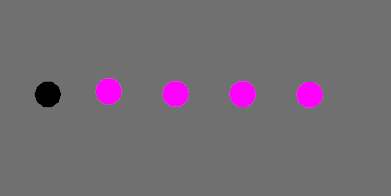
\includegraphics[width=3.5cm]{Images/cir_1.png} &
      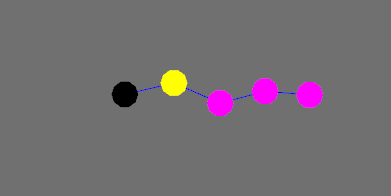
\includegraphics[width=3.5cm]{Images/cir_2.png} &
      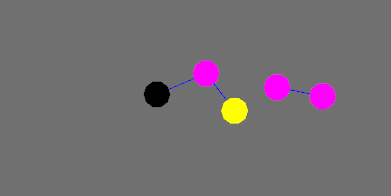
\includegraphics[width=3.5cm]{Images/cir_3.png} \\
      \hline
      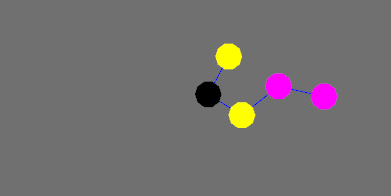
\includegraphics[width=3.5cm]{Images/cir_4.png} &
      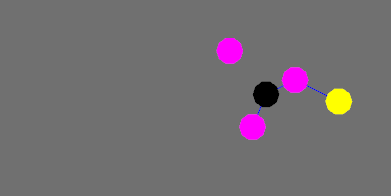
\includegraphics[width=3.5cm]{Images/cir_5.png} &
      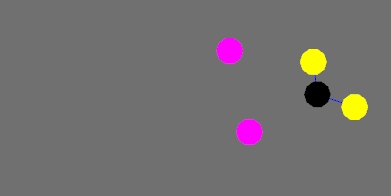
\includegraphics[width=3.5cm]{Images/cir_6.png} \\
      \hline
    \end{tabular}
    \end{center}
    \caption{Six échantillons de compressions avec le centre instantané de rotation.}
  \end{figure}
\end{frame}

\subsection{Compression et traction}
\begin{frame}{Loi de Hooke et module de Young}
  \begin{center}
    $\sigma = E \times \varepsilon$
  \end{center}
  $\sigma = $ Contrainte appliquée sur le matériau (en Pa). $E = $ Module de Young pour le matériau étudié (en Pa). $\varepsilon = $ Coefficient de déformation (en $\%$). \smallbreak
  Module de Young :
  \begin{itemize}
    \item Granite : 60 GPa ;
    \item Calcaire : 20 à 70 GPa.
  \end{itemize}
\end{frame}

\begin{frame}{Approximation de la compression et traction}
  Approximation symétrique dans les cas de compressions et tractions. \\
  Où $d'$ = $1 -$ la distance entre les deux cellules. \\
  \begin{center}
    Si traction : \medbreak
    \boxed{d' \leqslant 0 \Rightarrow \sigma = -d'^2} \medbreak
    Si compression : \medbreak
    \boxed{d' > 0 \Rightarrow \sigma = d'^2}
  \end{center}
\end{frame}

\begin{frame}{Démonstration de la compression et traction}
  \begin{figure}
  \subfigure[b][Sans compression]{
    \begin{tabular}{|M|M|}
      \arrayrulecolor{sky}
      \hline
      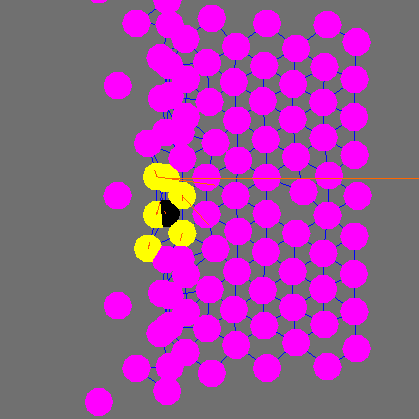
\includegraphics[width=2.4cm]{Images/normal_1.png} &
      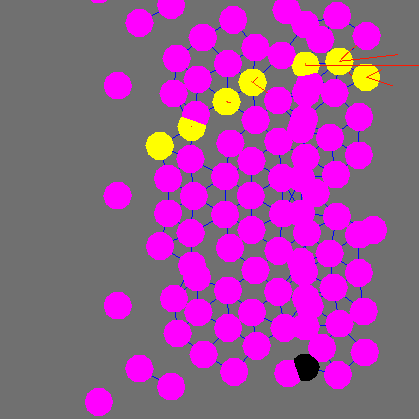
\includegraphics[width=2.4cm]{Images/normal_2.png} \\
      \hline
    \end{tabular}
  }
  \subfigure[Avec compression]{
    \begin{tabular}{|M|M|}
      \arrayrulecolor{sky}
      \hline
      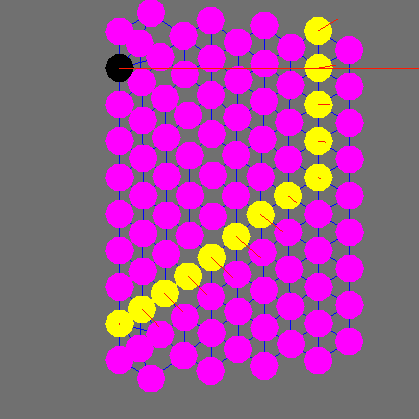
\includegraphics[width=2.4cm]{Images/compression_1.png} &
      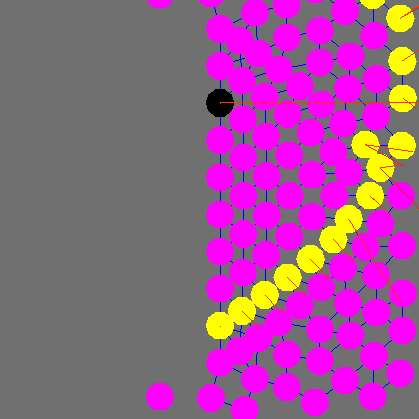
\includegraphics[width=2.4cm]{Images/compression_2.png} \\
      \hline
    \end{tabular}
  }
  \caption{Pair de deux échantillons de simulation avec et sans compression}
  \end{figure}
\end{frame}

\subsection{La propagation par fronts}
\begin{frame}{Front de cellules}
  Propagation par front, l’ancien front crée le nouveau. Le premier front ne contient que la cellule en collision.
  Chaque cellule du front interagit avec les cellules qui précèdent le front.
  \begin{figure}
    \begin{tabular}{|M|M|M|}
      \arrayrulecolor{sky}
      \hline
      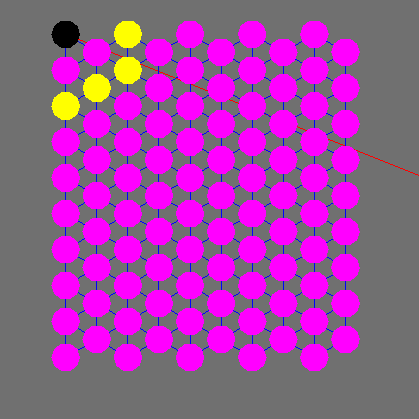
\includegraphics[width=2.5cm]{Images/front_1.png} &
      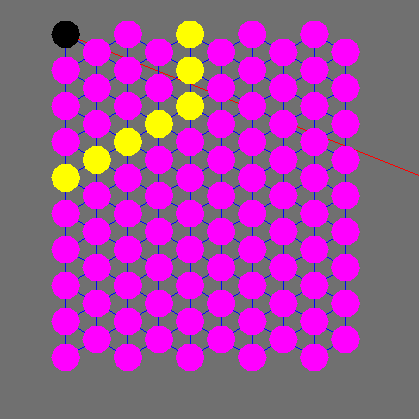
\includegraphics[width=2.5cm]{Images/front_2.png} &
      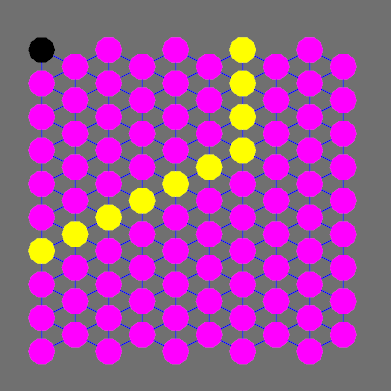
\includegraphics[width=2.5cm]{Images/front_3.png} \\
      \hline
      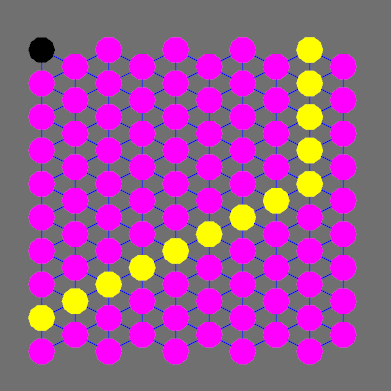
\includegraphics[width=2.5cm]{Images/front_4.png} &
      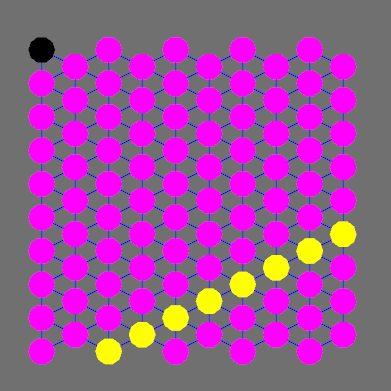
\includegraphics[width=2.5cm]{Images/front_5.png} &
      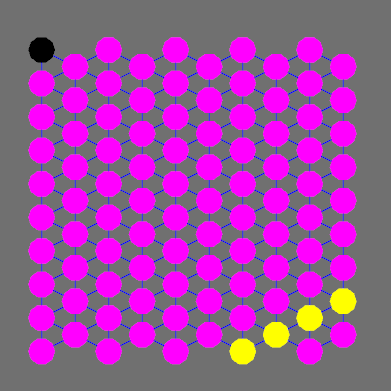
\includegraphics[width=2.5cm]{Images/front_6.png} \\
      \hline
    \end{tabular}
    \caption{Six échantillons de propagation de front lors de la simulation}
  \end{figure}
\end{frame}

\begin{frame}{Calques de vélocités}
  Utilisation d'un calque pour chaque cellule en collision. Fusion des calques avant le déplacement des cellules.
  \begin{figure}
    \begin{center}
      \includegraphics[width=6cm]{Images/calque.png}
    \end{center}
    \caption{Du rouge vers le jaune les différentes vélocités par cellules et par collisions.}
  \end{figure}
\end{frame}

\subsection{La friction}
\begin{frame}{Loi de Coulomb}
  \begin{center}
    $T_0 = f_0 \times N$
  \end{center}
  Si $T > T_0$ : glissement. Sinon friction. \smallbreak
  Où $T = $ : force tangentielle, $N = $ : contrainte à la normale, $f_0 = $ : coefficient d'adhérence.
  \begin{figure}
    \begin{center}
      \begin{tikzpicture}[line cap=round,line join=round,>=triangle 45,x=0.8cm,y=1.0cm]
	\clip(-4,-1) rectangle (4,2);
	\draw [shift={(0,0)},color=qqwuqq,fill=qqwuqq,fill opacity=0.1] (0,0) -- (53.13:0.63) arc (53.13:126.87:0.63) -- cycle;
	\draw (-1.5,2)-- (0,0);
	\draw (0,0)-- (1.5,2);
	\draw (1.5,2)-- (-1.5,2);
	\draw [domain=-4:4] plot(\x,{(-0-0*\x)/4});
	\draw (0,0)-- (0,1.41);
	\draw (-1.06,1.41)-- (1.06,1.41);
	\begin{scriptsize}
	  \draw[color=qqwuqq] (0.1,0.4) node {$f_0$};
	  \draw[color=black] (0.21,0.79) node {$N$};
	  \draw[color=black] (0.1,1.55) node {$T$};
	\end{scriptsize}
      \end{tikzpicture}
    \end{center}
    \caption{Le cône représentant la force maximale possible avant un glissement.}
  \end{figure}
\end{frame}

\subsection{Les limites matérielles}
\begin{frame}{Limites de temps de calcules}
  \begin{center}
    \begin{tikzpicture}
      \begin{axis}[height=5cm,width=10cm, axis x line=bottom, axis y line=left, grid=major, xlabel={Nombre de cellules}, ylabel={Temps de calcul (en ms)}]
	\addplot coordinates {
	  (100,2.5)
	  (2500,41)
	  (10000,167)
	  (22500,366)
	  (40000,654)
	  (62500,1010)
	  (90000,1466)
	};
      \end{axis}
    \end{tikzpicture}
  \end{center}
  \begin{center}
    \boxed{1.629 \times 10^{-2} ms/cellule}
  \end{center}
  $100 \times 10^2 \times 100 \times 10^2 \times 10 \times 10^2 = 10^{11}$ cellules \\
  100 milliards de cellules : $16290000000$ ms = 4525 h = 189 j\\
  $10000$ cellules en collisions : 1890000 j = 5178 a.
\end{frame}

\section{Les Améliorations possibles}
\begin{frame}{Améliorations possibles de la simulation}
  Améliorations au profit du réalisme :
  \begin{itemize}
    \item implémenter les altérations~;
    \item implémenter la loi de Hooke et la loi de Coulomb~;
    \item implémenter l'inertie.
  \end{itemize}
  Améliorations au profit de l'optimisation~:
  \begin{itemize}
    \item regrouper certaines cellules de vecteurs~;
    \item paralléliser les calculs (accélération graphique).
  \end{itemize}
\end{frame}

\section{Conclusion}

\subsection{Remerciements et sources}
\begin{frame}{Sources}
  \begin{footnotesize}
  \begin{itemize}
   \item Richard Bézin, Benoît Crespin, Xavier Skapin, Olivier Terraz, Philippe Meseure. Opérations
topologiques pour la géomorphologie.
    \begin{tiny} 
     Journées de l’Association Française d’Informatique Graphique, Oct 2011, Biarritz, France. pp.95-104, 2011. $<hal-00633705>$
    \end{tiny}
   \item Pascale Roudier. Synthèse de paysages réalistes par simulation de processus d’érosion. 
    \begin{tiny}
    Graphics
[cs.GR]. École Nationale Supérieure des Mines de Saint-Etienne; Université Jean Monnet -
Saint-Etienne, 1993. French. $<NNT : 1993STET4011>. <tel-00835373>$
	\end{tiny}
   \item Thomas Leduc. Modélisation par un système dynamique discret du processus de subduction-érosion en tectonique des plaques : première approche uni-dimensionnelle. 
    \begin{tiny}
    Laboratoires LIP6, Mai 1997.
    \end{tiny}
   \item Thomas Leduc. Modélisations par réseaux d’automates cellulaires et simulations parallèles
du phénomène de subduction- érosion en tectonique des plaques. 
     \begin{tiny}
     Modeling and Simulation.
Université Pierre et Marie Curie - Paris VI, 1999. French. $<tel-00327733>$
	 \end{tiny}
   \item Thomas Leduc. Simulation par automates cellulaires bi-dimensionnels en géotectonique. 
     \begin{tiny}
     Laboratoires LIP6, 1999.
     \end{tiny}
%    \item Wikipédia (lois et algorithmes) et Google Images (Illustrations)
  \end{itemize}
% Il est obligé de citer ainsi les thèses d'un point de vue légal. Ceci dit, la taille des informations inutiles sera réduite au minimum pour plus de clarté.
  \end{footnotesize}
\end{frame}

\begin{frame}{Sources Wikipédia}
  \begin{footnotesize}
    \begin{itemize}
      \item Loi de Hooke~:
	\begin{tiny}
	  \url{https://fr.wikipedia.org/wiki/Loi_de_Hooke}
	\end{tiny}
      \item Module de Young~:
	\begin{tiny}
	  \url{https://fr.wikipedia.org/wiki/Module_de_Young}
	\end{tiny}
      \item Loi de Coulomb~:
	\begin{tiny}
	  \url{https://fr.wikipedia.org/wiki/Loi_de_Coulomb_(mecanique)}
	\end{tiny}
    \end{itemize}
  \end{footnotesize}
\end{frame}

\end{document}
